\documentclass[svgnames,11pt]{beamer}
\input{/home/tof/Documents/Cozy/latex-include/preambule_commun.tex}
\input{/home/tof/Documents/Cozy/latex-include/preambule_beamer.tex}
%\usepackage{pgfpages} \setbeameroption{show notes on second screen=left}
\author[]{Christophe Viroulaud}
\title{Gestion d'une collection de bandes-dessinées\\Modèle relationnel}
\date{\framebox{\textbf{BDD 01}}}
%\logo{}
\institute{Terminale - NSI}

\begin{document}
\begin{frame}
    \titlepage
\end{frame}
\begin{frame}
    \frametitle{}

    Pour gérer son importante collection de bandes-dessinées, les nouveautés mais également les emprunts, le professeur veut s'appuyer sur un modèle informatique.
    \begin{center}
        \centering
        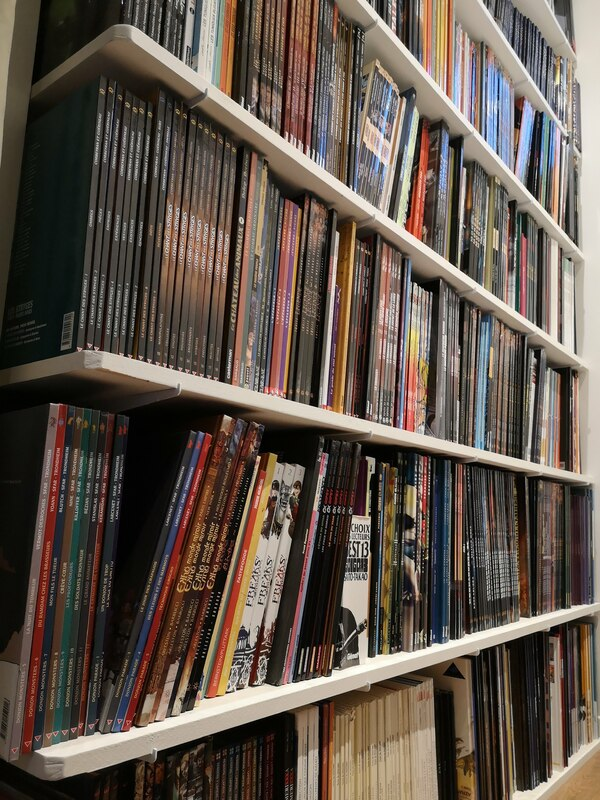
\includegraphics[width=4.5cm]{ressources/biblio.jpg}
        \captionof{figure}{Extrait de la collection}
        \label{IMG}
    \end{center}

\end{frame}
\begin{frame}
    \frametitle{}

    \begin{framed}
        Quelle solution mettre en place pour gérer efficacement une grande quantité de données?
    \end{framed}

\end{frame}
\section{Solution naïve: le tableur}
\begin{frame}
    \frametitle{Solution naïve: le tableur}

    \begin{center}
        \centering
        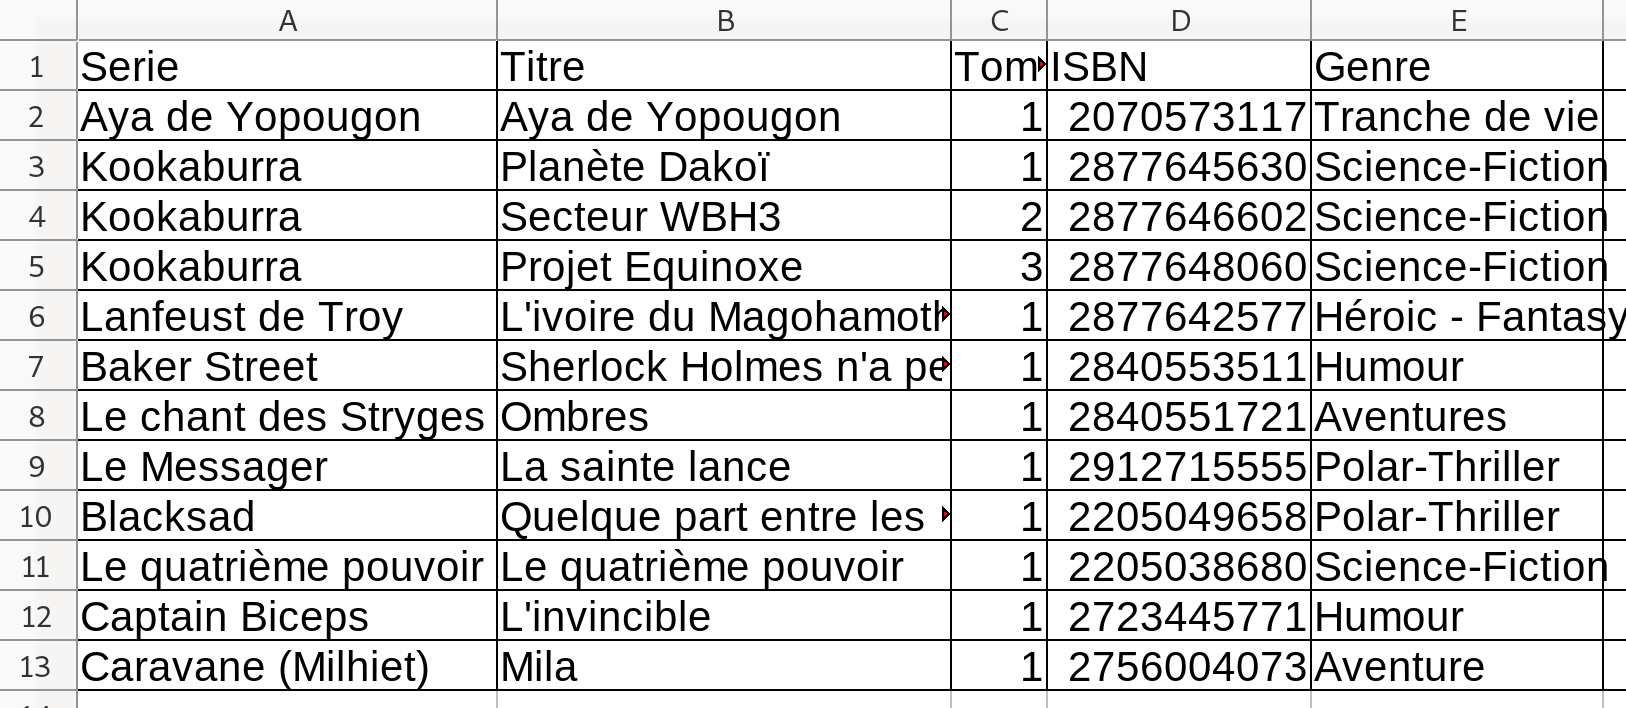
\includegraphics[width=10cm]{ressources/approche-1.png}
        \captionof{figure}{Utilisation d'un fichier \textbf{\texttt{CSV}}}
        \label{IMG}
    \end{center}
    \begin{activite}
        Établir les limites de cette approche.
    \end{activite}
\end{frame}
\begin{frame}
    \frametitle{Correction}
    \begin{center}
        {\Large Gestion de grandes quantités de données}\\
        \href{https://www.numerama.com/politique/653217-16-000-anglais-malades-du-covid-ont-ete-oublies-a-cause-dune-feuille-excel-trop-pleine.html}{
\includegraphics[width=8cm]{ressources/oublies.png}}
    \end{center}
\end{frame}
\begin{frame}
    \frametitle{}

    \begin{center}
        {\Large Gestion efficace des modifications\\ $\rightleftarrows$ redondance}
    \end{center}
    \begin{center}
        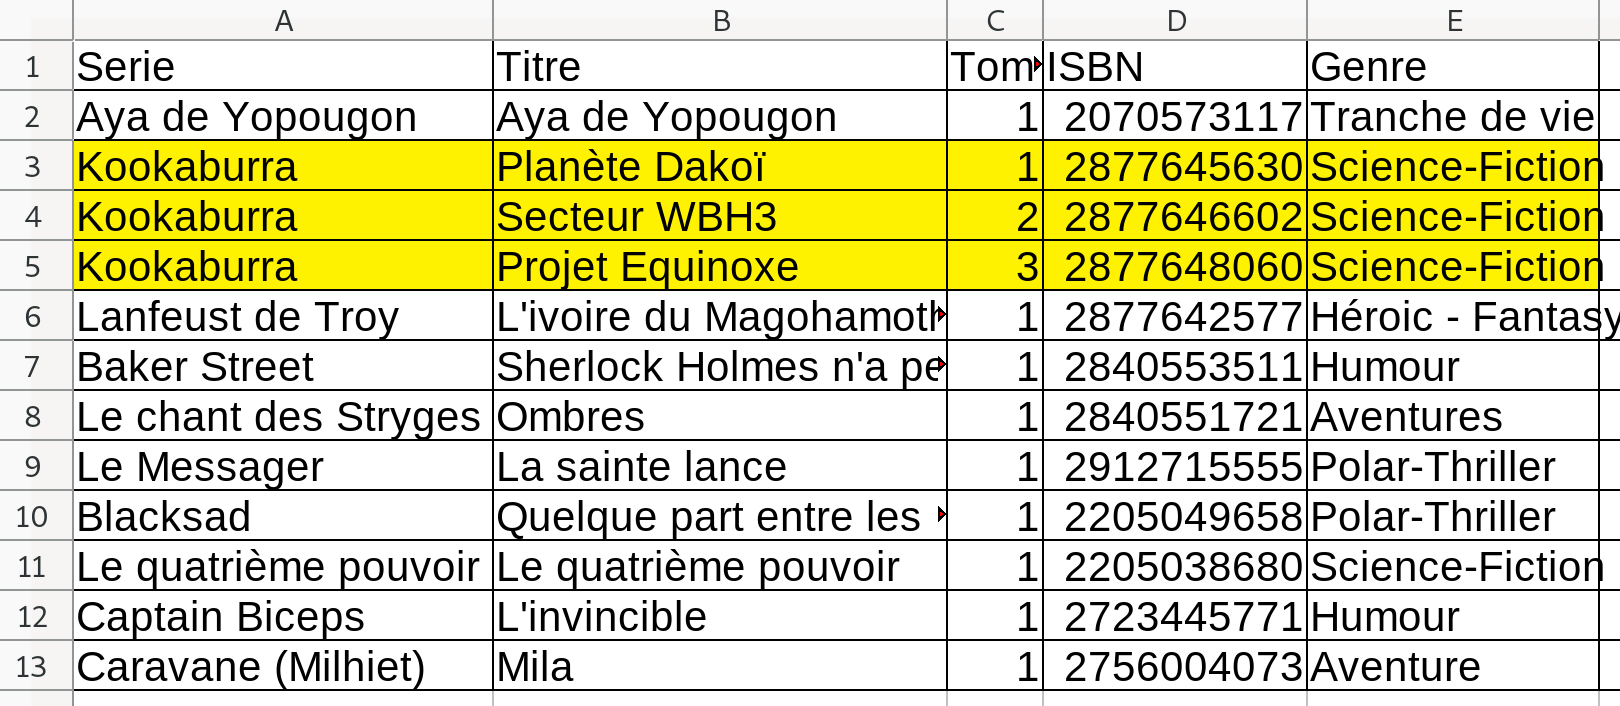
\includegraphics[width=10cm]{ressources/approche-11.png}
    \end{center}
\end{frame}
\begin{frame}
    \frametitle{}

    \begin{center}
        {\Large Gestion des informations \emph{externes}}
    \end{center}
    \begin{center}
        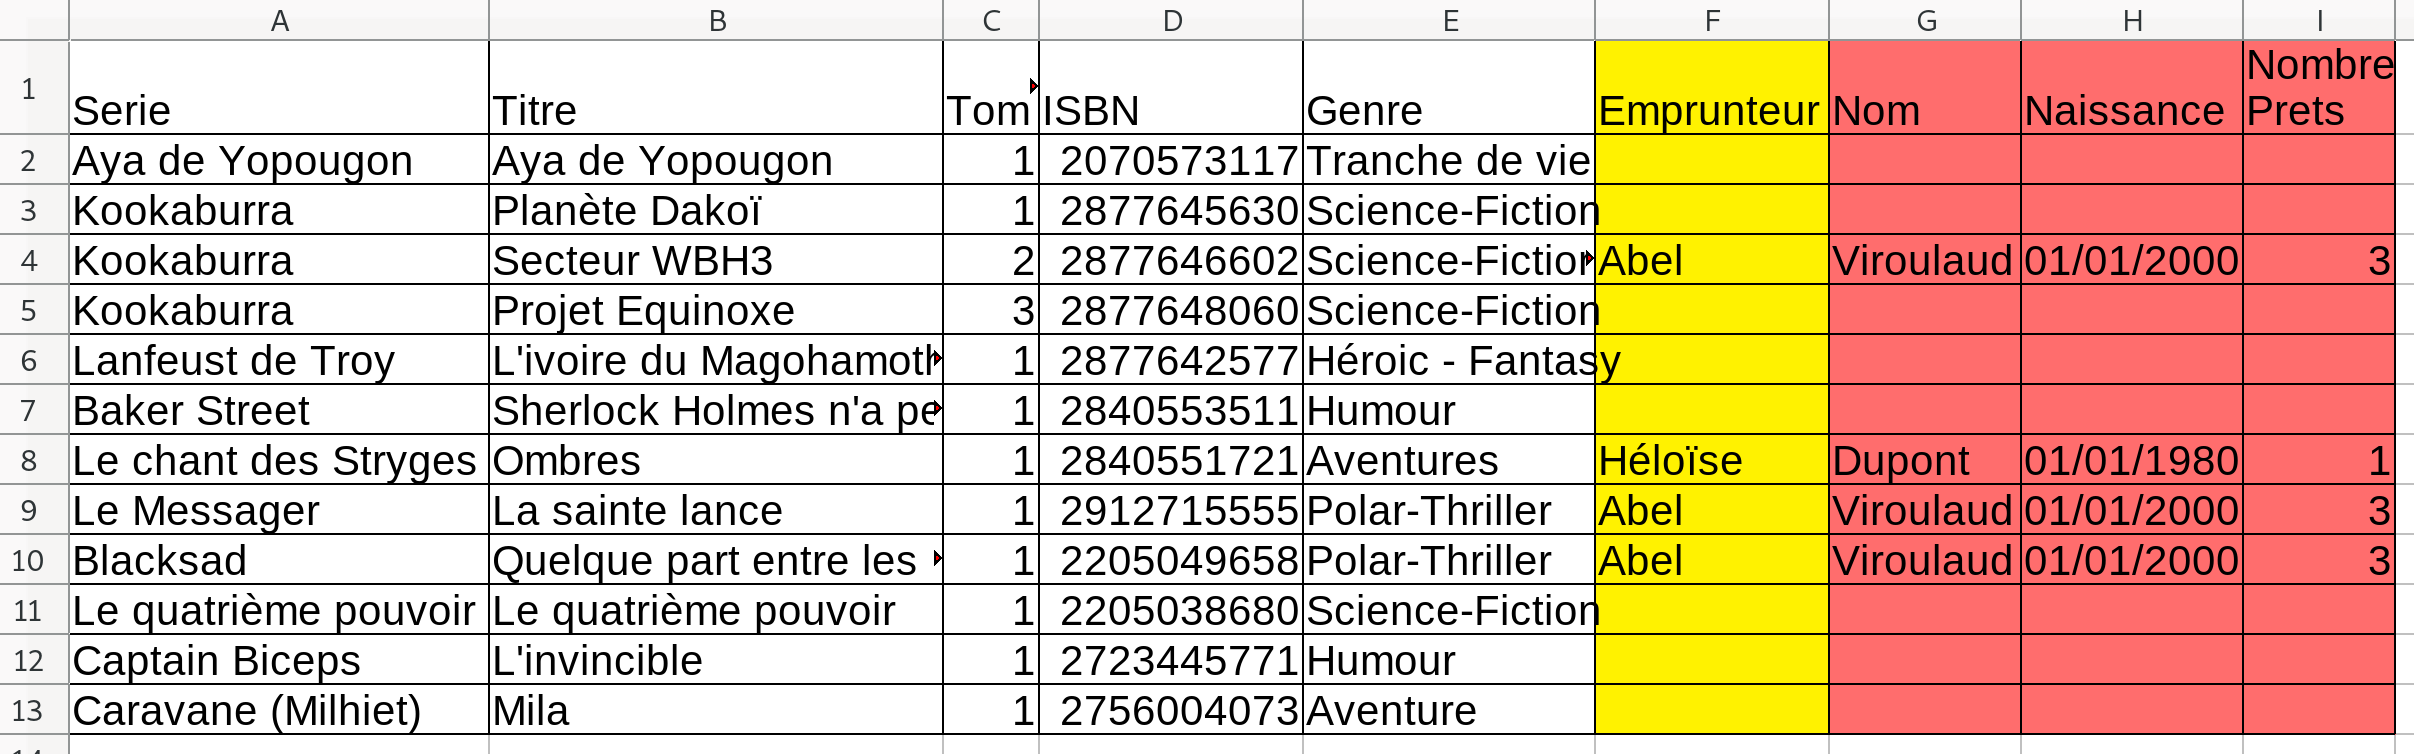
\includegraphics[width=10cm]{ressources/approche-12.png}
    \end{center}
\end{frame}
\section{Modèle relationnel}
\begin{frame}
    \frametitle{Modèle relationnel}

    \begin{aretenir}[]
        Une \textbf{entité} est un objet représenté par un n-uplet de valeurs scalaires.
    \end{aretenir}
    Une bande dessinée est une entité :
    \begin{center}
        (Captain Biceps, L’invincible, 1, 2723445771, Humour)
    \end{center}
\end{frame}
\begin{frame}
    \frametitle{}

    \begin{aretenir}[]
        Une \textbf{relation} est un tableau à deux dimensions qui regroupe l'ensemble des entités.\\    Une relation possède des \textbf{attributs}.

    \end{aretenir}
    La relation \emph{Bandes\_dessinees} possède les attributs:
    \begin{center}
        (serie, titre, tome, isbn, genre)
    \end{center}
\end{frame}
\begin{frame}
    \frametitle{}

    \begin{center}
        \begin{tabular}{|*{5}{c|}}
            \hline
            serie          & titre           & tome & isbn       & genre    \\
            \hline
            Captain Biceps & L’invincible    & 1    & 2723445771 & Humour   \\
            Caravane       & Mila            & 1    & 2756004073 & Aventure \\
            Kick-Ass       & Le premier\dots & 1    & 2809409994 & Comics   \\
            \hline
        \end{tabular}
        \captionof{table}{Relation \emph{Bandes\_dessinees}}
    \end{center}

    \begin{center}
        \begin{tabular}{|*{3}{c|}}
            \hline
            nom       & prenom  & naissance  \\
            \hline
            Viroulaud & Abel    & 2000-01-01 \\
            Dupont    & Héloïse & 1980-01-01 \\
            \hline
        \end{tabular}
        \captionof{table}{Relation \emph{Emprunteurs}}
    \end{center}
    \begin{aretenir}[Remarque]
        Les relations peuvent interagir entre elles.
    \end{aretenir}
\end{frame}
\section{Contraintes d'intégrité}
\begin{frame}
    \frametitle{Contraintes d'intégrité}

    \begin{aretenir}[]
        Une contrainte d’intégrité est une propriété vérifiée à tout instant et qui garantit la cohérence des
        données.
    \end{aretenir}

\end{frame}
\subsection{Contrainte de domaine}
\begin{frame}
    \frametitle{Contrainte de domaine}

    Chaque propriété que l'on souhaite renseigner est représentée par un \emph{attribut} dans une relation. 
    \begin{aretenir}[]
        Le \textbf{domaine de définition} de chaque attribut doit garantir qu'il n'y aura pas de perte de données.
    \end{aretenir}

\end{frame}
\begin{frame}
    \frametitle{}

    \begin{center}
        \begin{tabular}{|cc|}
        \hline 
        \multicolumn{2}{|c|}{Bandes\_dessinees} \\ 
        \hline 
        serie & String \\ 
        titre & String \\ 
        tome & Integer \\ 
        isbn & Integer \\ 
        genre & String \\ 
        \hline 
        \end{tabular} 
        \captionof{code}{\textbf{Schéma} de la relation bandes\_dessinees}
        \end{center}
        Une autre manière de présenter le schéma:
        
        Bandes\_dessinees(serie \emph{String}, titre \emph{String}, tome \emph{Integer}, isbn \emph{String}, genre \emph{String})

\end{frame}
\begin{frame}
    \frametitle{}

    \begin{activite}
        Ajouter l'attribut \emph{telephone} dans la relation \textbf{Emprunteurs}. Quel domaine de définition semble le plus approprié?
        \end{activite}

\end{frame}
\begin{frame}
    \frametitle{Correction}

    Emprunteurs(nom \emph{String}, prenom \emph{String}, naissance \emph{String}, telephone \emph{String})

    exemples de numéro:
    \begin{itemize}
        \item 0601020301
        \item +3323019239
    \end{itemize}
\end{frame}
\subsection{Contrainte d'intégrité}
\begin{frame}
    \frametitle{Contrainte d'intégrité}

    \begin{aretenir}[]
        La \textbf{contrainte d'intégrité} garantit que chaque entité d'une relation est \emph{unique} et l'identifie de manière non ambiguë.
    \end{aretenir}

\end{frame}
\begin{frame}
    \frametitle{}

    \begin{center}
        \begin{tabular}{|*{5}{c|}}
            \hline
            serie          & titre           & tome & isbn       & genre    \\
            \hline
            Captain Biceps & L’invincible    & 1    & 2723445771 & Humour   \\
            Caravane       & Mila            & 1    & 2756004073 & Aventure \\
            Kick-Ass       & Le premier\dots & 1    & 2809409994 & Comics   \\
            \hline
        \end{tabular}
        \captionof{table}{Relation \emph{Bandes\_dessinees}}
    \end{center}
    \begin{activite}
        Dans la relation \emph{Bandes\_dessinees}, y-a-t-il un attribut qui garantit cette contrainte?
    \end{activite}
\end{frame}
\begin{frame}
    \frametitle{}

    L'ISBN est un numéro unique.

    \begin{aretenir}[]
        On appelle \textbf{clé primaire} l'attribut qui garantit l'unicité de l'entité.
        \end{aretenir}
        On indique la \emph{clé primaire} en la soulignant dans le schéma:\\
\begin{center}
    Bandes\_dessinees(serie \emph{String}, titre \emph{String}, tome \emph{Integer}, \underline{isbn \emph{String}}, genre \emph{String})
\end{center}

\end{frame}
\begin{frame}
    \frametitle{}

    \begin{activite}
    Donner une clé primaire pour la table \textbf{Emprunteurs}.
    \end{activite}
    \begin{center}
        \begin{tabular}{|*{3}{c|}}
            \hline
            nom       & prenom  & naissance  \\
            \hline
            Viroulaud & Abel    & 2000-01-01 \\
            Dupont    & Héloïse & 1980-01-01 \\
            \hline
        \end{tabular}
        \captionof{table}{Relation \emph{Emprunteurs}}
    \end{center}
\end{frame}
\begin{frame}
    \frametitle{}

    Emprunteurs(\underline{nom \emph{String}, prenom \emph{String}}, naissance \emph{String})

    \begin{aretenir}[Remarque]
    Une clé primaire peut être composite. 
    \end{aretenir}
\end{frame}
\begin{frame}
    \frametitle{}

    Dans notre cas cette clé n'est pas suffisante: il existe des homonymes. Il faut définir un nouvel attribut.
    \begin{center}
        Emprunteurs(\underline{id \emph{Integer}}, nom \emph{String}, prenom \emph{String}, naissance \emph{String})
    \end{center}

\end{frame}
\subsection{Contrainte de référence}
\begin{frame}
    \frametitle{Contrainte de référence}

    \begin{activite}
    Créer la relation \textbf{Emprunts} qui permet de gérer les emprunts de bandes-dessinées par les emprunteurs.
    \begin{itemize}
        \item Bandes\_dessinees(serie \emph{String}, titre \emph{String}, tome \emph{Integer}, \underline{isbn \emph{String}}, genre \emph{String})
        \item Emprunteurs(\underline{id \emph{Integer}}, nom \emph{String}, prenom \emph{String}, naissance \emph{String})
    \end{itemize}
    \end{activite}

\end{frame}
\begin{frame}
    \frametitle{Correction}

    \begin{center}
        Emprunts(\underline{isbn String}, id\_emprunteurs Integer)
    \end{center}

    \begin{aretenir}[Remarque]
    Un emprunteur peut prendre plusieurs bandes-dessinées. Par contre il n'y a qu'un exemplaire de chaque bande-dessinée dans la bibliothèque.
    \end{aretenir}
\end{frame}
\begin{frame}
    \frametitle{}

    \begin{aretenir}[]
        La contrainte de référence garantit qu'une entité d'une relation B mentionne une entité existante dans une relation A.
    \end{aretenir}

    Dans la relation \textbf{Emprunts}, l'isbn doit référencer une bande-dessinée existante. Il en est de même pour l'identifiant de l'emprunteur.
\end{frame}
\begin{frame}
    \frametitle{}

    \begin{aretenir}[]
        Une \textbf{clé étrangère} est une référence à une clé primaire d'une autre relation. Elle garantit:
        \begin{itemize}
        \item que la valeur de l'attribut crée dans la relation existe dans la relation liée,
        \item qu'on ne peut supprimer une entité si elle est liée à une autre relation.
        \end{itemize}
    \end{aretenir}
    On note une clé étrangère par un trait pointillé.
\begin{center}
    Emprunts(\underline{\dashuline{isbn Integer}}, \dashuline{id\_emprunteurs Integer})
\end{center}
\end{frame}
\section{Base de données}
\begin{frame}
    \frametitle{Base de données}

    \begin{aretenir}[]
    L'ensemble des relations constitue une \textbf{base de données}.
    \end{aretenir}
\begin{center}
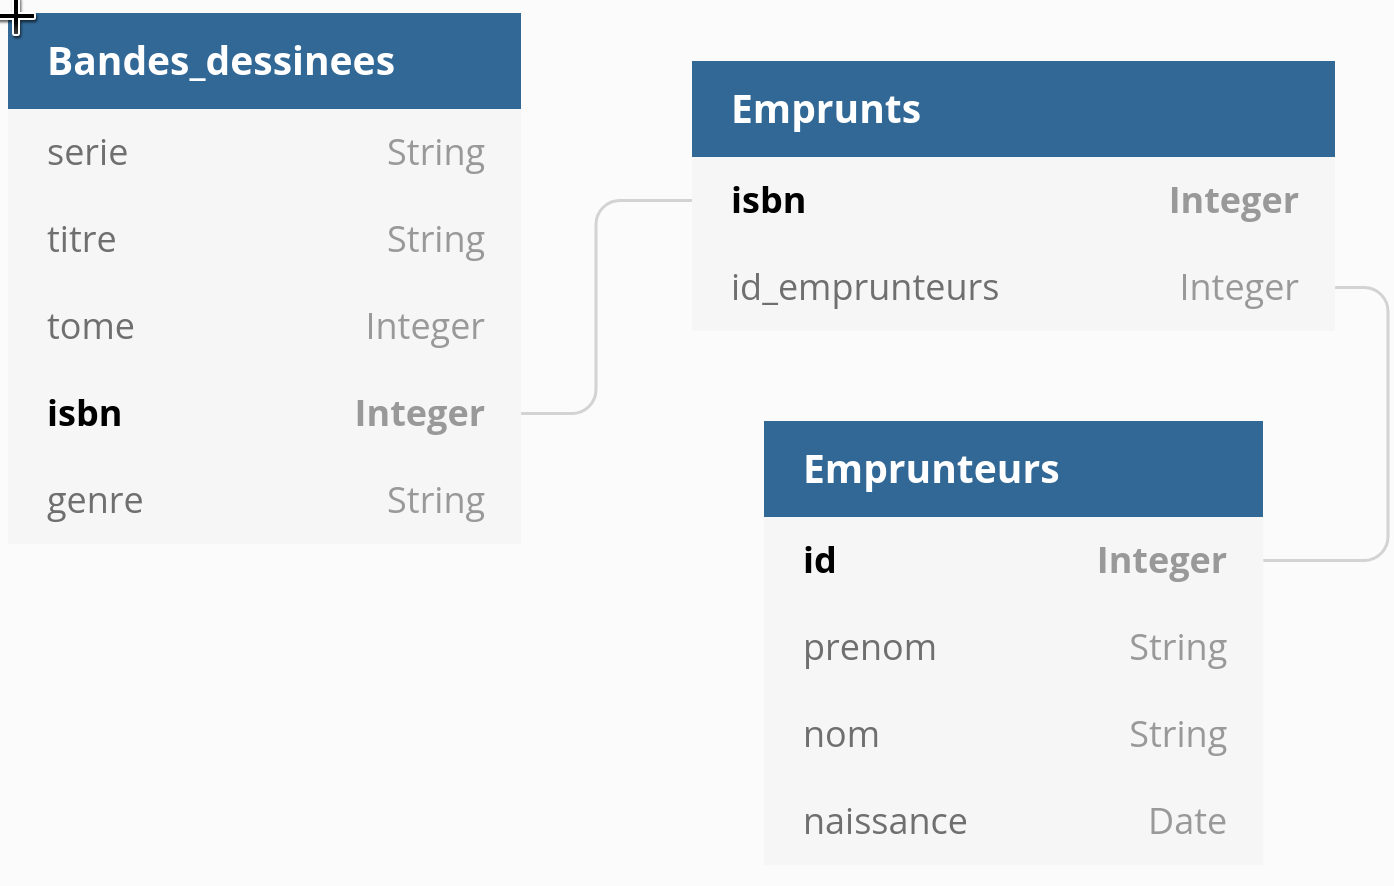
\includegraphics[width=10cm]{ressources/etrangere.png}
\end{center}
\end{frame}
\begin{frame}
    \frametitle{}

    \begin{center}
    \centering
    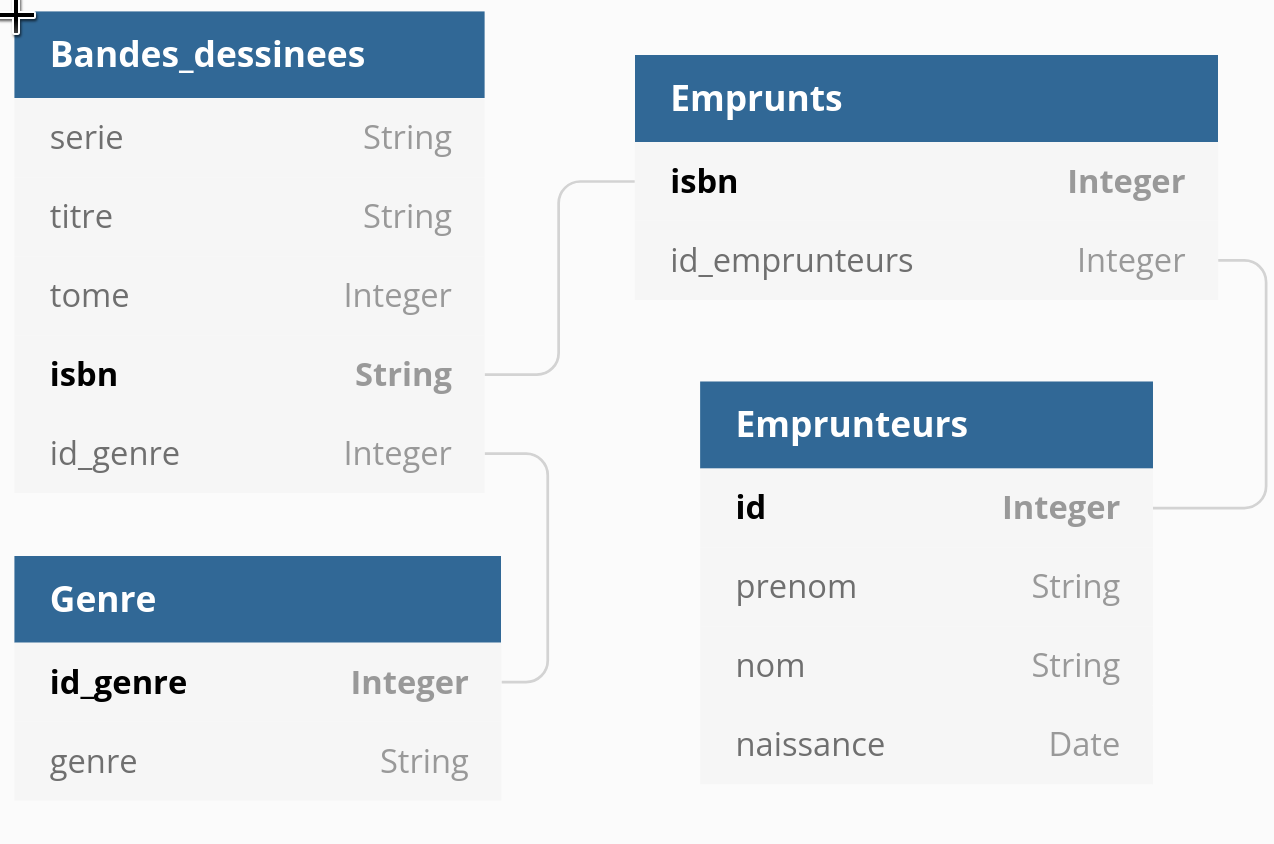
\includegraphics[width=10cm]{ressources/etrangere-2.png}
    \captionof{figure}{Une amélioration de la base}
    \label{IMG}
    \end{center}

\end{frame}
\end{document}